\documentclass[12pt,journal]{IEEEtran}

\usepackage{footmisc}
\usepackage[hidelinks]{hyperref}
\usepackage[T1]{fontenc}
\usepackage[utf8]{inputenc}
\usepackage{listings}
\usepackage{graphicx}
\usepackage{dblfloatfix}
\usepackage{caption}
\usepackage{minted}
\captionsetup{font=footnotesize}

% Keywords command
\providecommand{\keywords}[1]
{
  \small	
  \textbf{\textit{Sleutelwoorden---}} #1
}

\graphicspath{ {../images/} }
\begin{document}
\pagestyle{empty}
\title{Jaarplannen van leerkrachten voorstellen met RDF}
\author{Michiel Rogissart\\[12pt]
	\large Promotor: Thomas Delva \\
	Co-promotoren: Dr. ir. Ben de Meester, Prof. dr. Kris Coolsaet}
\maketitle

\pagenumbering{roman}

\setcounter{page}{7}
\thispagestyle{plain}
\pagestyle{plain}
\begin{abstract}
	Een van de voordelen van linked data is dat het inzichtelijke informatie over data mogelijk maakt, met minder complexe queries dan bijvoorbeeld SQL\cite{sqlvsqparql}.
	Dit voordeel kan worden benut door leerkrachten die een goed inzicht willen in hun jaarplan. Een jaarplan is de verzameling van alle lessen die een leraar gedurende een schooljaar geeft.
	Het bijhouden van bepaalde eigenschappen van lessen, zoals interactiviteit en behandelde competenties, kan nu een hele uitdaging zijn.
	Daardoor houden niet veel leerkrachten deze eigenschappen daadwerkelijk bij.
	Er bestaan applicaties om leraren te helpen, maar ze hebben een aantal problemen vanwege hun gecentraliseerde karakter.\\
	Dit onderzoek stelt een gelinkt datamodel voor, voor het modelleren van jaarplannen. Het doel is om veel bruikbare inzichten te bieden over jaarplannen, zonder leerkrachten te belasten met zelf veel gegevens in te voeren.
	Het model is gemaakt met behulp van de `eXtreme Design'-methodologie \cite{xd}.
	Om dit te bereiken werde competentievragen afgeleid uit interviews met domeinexperten.
	Elke competentievraag heeft een bijbehorende SPARQL-query, wat suggereert dat dit model functioneel is voor deze toepassing.
	\keywords{Gelinkte data, Onderwijs, RDF Ontologie}
\end{abstract}

\section{Introductie en doelstelling}
\noindent Het doel van dit onderzoek is het ontwikkelen van een gelinkt datamodel dat jaarplannen representeert. Dit moet gebeuren op basis van de behoeften van leerkrachten.
	Meer specifiek is het belangrijk om belangrijke aspecten van jaarplannen te identificeren die op een overzichtelijke manier aan leerkrachten kunnen worden gepresenteerd. \\ \\
	Granulariteit, dataconsistentie en hergebruik van bestaande ontologieën zijn sleutelbegrippen bij het ontwikkelen van dit model om een duurzaam resultaat te garanderen.\\
	Een analyse van de bestaande applicaties, en wat leerkrachten denken dat deze missen, is ook belangrijk. Vooral de problemen die voortkomen uit het gecentraliseerde karakter.
	In de volgende paragraaf worden deze bestaande applicaties en hun problemen besproken.

	\subsection{Bestaande applicaties}
	\label{subsection:existing-tools}
	\noindent De meeste onderwijsgerichte applicaties focussen op het verlichten van de administratieve taken van een leerkracht door een interface aan te bieden om taken te communiceren, beoordelen en bij te houden.
	Applicaties zoals Google Classroom \footnote{https://edu.google.com/intl/ALL\_nl/workspace-for-education/classroom/} en Planboard \footnote{https://www.chalk.com/planboard/} bieden deze functionaliteiten aan.\\
	Een andere belangrijke applicatie, zeker voor het Vlaams onderwijs \cite{destandaard}, is Smartschool \footnote{https://www.smartschool.be/}.\\
	Dit is een online leerplatform dat onder andere functionaliteit biedt om lesvoorbereidingen bij te houden.\\ \\
	Belangrijke problemen die terugkomen bij deze applicaties staan hieronder opgesomd.
	\begin{itemize}
		\item Het linken van oefeningen en lessen aan de competenties die zij behandelen, is niet mogelijk of is heel gelimiteerd.
  		\item Omdat alle data op servers staat die eigendom zijn van een bedrijf, kan niemand de nodige applicaties gebruiken als deze servers zouden falen. Wanneer de data lekt, wordt data gelekt over een hele grote groep leerlingen.
    	\item De meeste applicaties zijn gemaakt voor de Verenigde Staten en zijn amper bruikbaar voor leerkrachten in andere landen.
     	\item Er wordt niet veel inzichtelijke informatie aangeboden, enkel de behandelde competenties. Interactiviteit, gebruike materialen worden niet bijgehouden.
      	\item Er is geen of nauwelijks functionaliteit om de gebruikte materialen te linken aan lessen.
       	\item De granulariteit is gelimiteerd tot het niveau van lessen. Dit maakt het ingewikkelder om delen van lessen te verplaatsen naar andere lessen.
        \item Leerkrachten moeten de meeste data zelf ingeven en kunnen geen gebruik maken van verschillende bronnen. Een leerkracht zou zich bijvoorbeeld niet hoeven bezighouden met het creëren van metadata over een leerboek dat gemaakt werd door een uitgever.  
	\end{itemize} 

\section{Materiaal en methodologie}
\noindent In dit deel worden de gebruikte technologieën en de methodolgie verder toegelicht.
	\subsection{Gebruikte materialen}
	\noindent Hier worden de gebruikte technologieën toegelicht. Zowel de gebruikte ontologieën, als enkele relevante databronnen, worden besproken.
		\subsubsection{Bestaande ontologieën}
		Dit model is vooral gebouwd op Schema.org \cite{schema}. Dit biedt al heel wat klassen en eigenschappen aan voor een educatieve context.
		Vooral de klasse \textit{schema:CreativeWork} werd vaak gebruikt.\\
		Educatief materiaal gebruikt in lessen (zoals handboeken), werden gemodelleerd met ontologieën van DC \cite{dc}.
		Meer bepaald \textit{bibo} \cite{bibo} en \textit{dcterms} \cite{dcterms}.
		Deze ontologieën bieden meer granulariteit in het beschrijven van documenten dan Schema.org.\\ \\
		Deze ontologieën implementeren de IEEE LOM (Learning Object Metadata) standaard \cite{ieeelom}.
		
		\subsubsection{Databronnen}
		De Vlaamse regering publiceerde gelinkte data \cite{ilearnskosmos} over de competenties, studierichtingen en curricula binnen het Vlaamse educatieve systeem met behulp van de skos ontologie.\\
		Dit werd verwezenlijkt vanuit het i-Learn project \footnote{https://www.i-learn.vlaanderen}. \\
		Een andere verwezenlijking van het i-Learn project, is een standaard woordenschat \cite{pubelovoc} dat gebruikt hoort te worden bij het creëren van metadata over lerenden.
		Ze stellen ook een metadataprofiel \cite{pubelo} voor, gebaseerd op IEEE-LOM.\\ \\
		Een andere vermeldingswaardige databron is een JSON API \footnote{https://onderwijs-vlaanderen-portaalov.apigee.io/apis} met dezelfde data als de skos databron, maar niet in een gelinkte data formaat.

	\subsection{Methodologie}
	\noindent De `eXtreme Design'-methodologie \cite{xd} werd gevolgd om dit model te ontwikkelen. Deze methodologie biedt een stappenplan aan om een ontologie te ontwikkelen gebaseerd op de noden van de gebruiker.
	Dit stappenplan wordt voorgesteld in figuur \ref{fig:xd-diagram}.
	
	\begin{figure}
		\caption[Extreme Design roadmap]{Stappenplan eXtreme Design zoals vermeld in \cite{xd}}
		\centering
		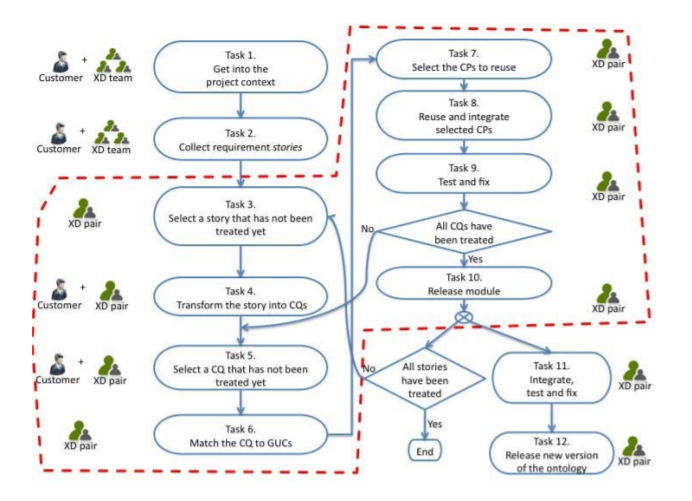
\includegraphics[scale=0.75]{xd-diagram.PNG}
		\label{fig:xd-diagram}
	\end{figure}
	\noindent Om de behoeften van de gebruiker in kaart te brengen, worden interviews afgenomen met domeinexperts. Deze interviews worden verwerkt tot behoefteverhalen: concrete verhalen over hoe iemand het model zou gebruiken.\\
	Deze behoefteverhalen werden vertaald naar competentievragen. Dit zijn concrete vragen die een gebruiker kan stellen over de data.
	Contextuele stellingen worden toegevoegd om ontwikkelaars te helpen de data te begrijpen (waar zij geen expert in zijn).\\
	Deze competentievragen worden vervolgens geïmplementeerd door het model te uit te breiden en SPARQL-query's te construeren die ze beantwoorden.

\section{Resultaten en discussie}
\noindent Het resulterende model wordt in deze sectie besproken. Het is opgedeeld in verschillende aspecten om het overzicht te behouden.
	\subsection{Competenties}
	\noindent Competenties zijn gemodelleerd zoals voorgesteld in figuur \ref{fig:uml-comp}.
	
	\begin{figure}[h]
		\caption{Modelleren van competenties}
		\label{fig:uml-comp}
		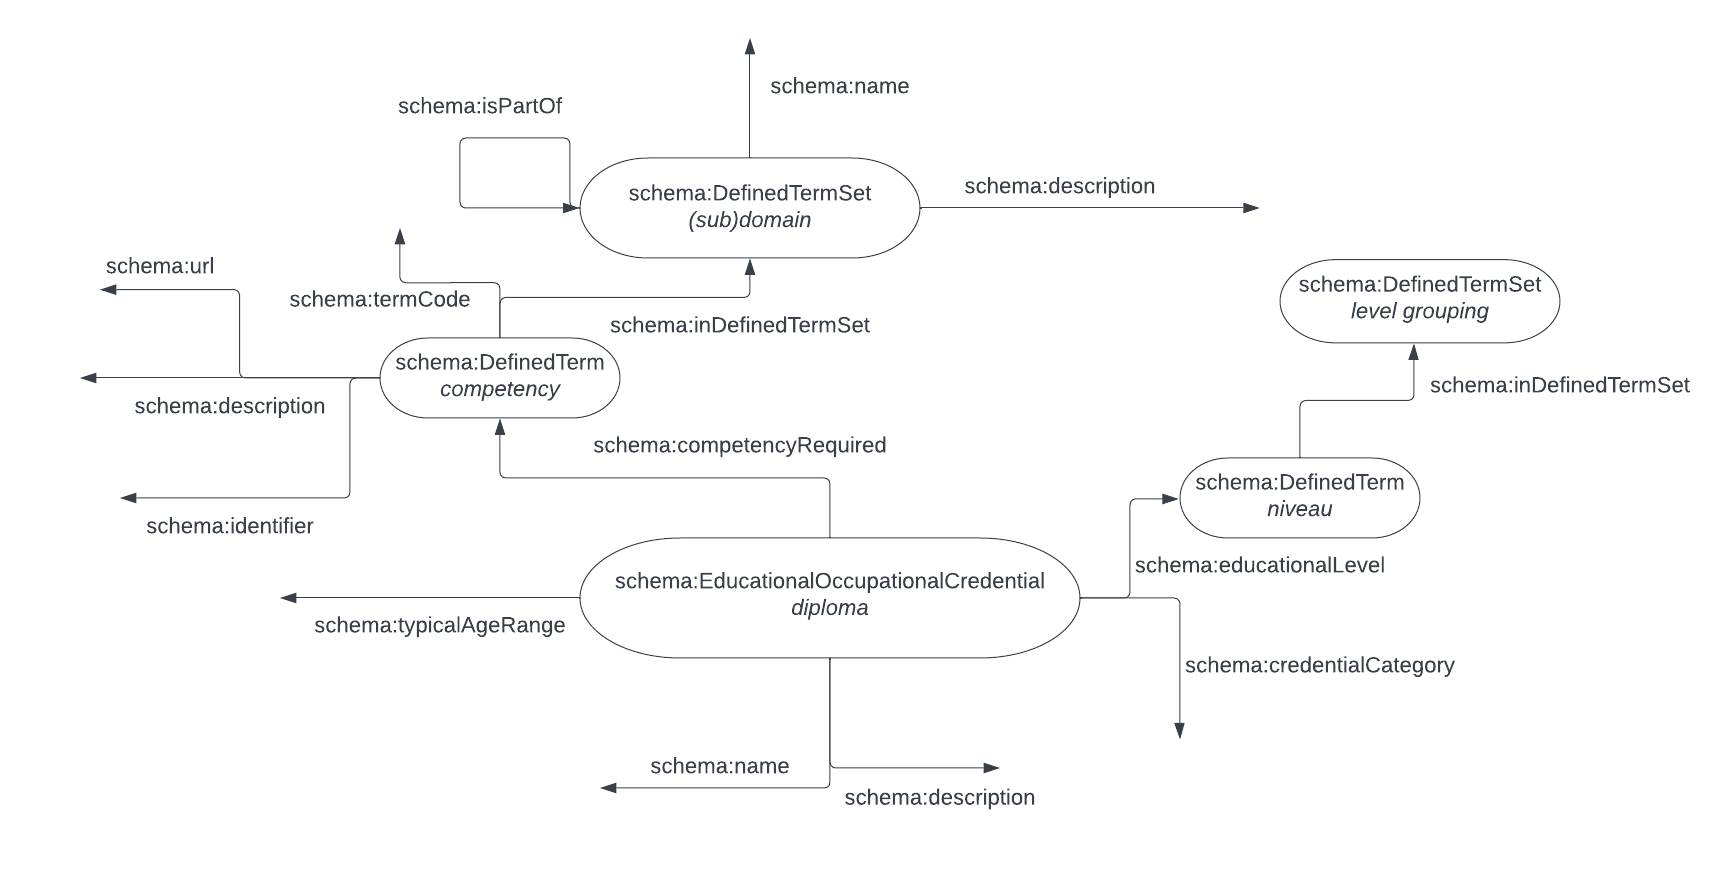
\includegraphics[scale=0.3]{uml-competencies.png}
	\end{figure}
	\noindent Ze worden voorgesteld door de klasse \textit{schema:DefinedTerm}. Dit maakt het onafhankelijk van de ontologie die door de overheid wordt gebruikt om deze gegevens vrij te geven.\\
	Competenties zijn doorgaans gegroepeerd in domeinen. Dit werd gedaan via de klasse \textit{schema:DefinedTermSet}.\\ \\
	Het onderwijsniveau dat een leerling heeft gekozen, is ook gemodelleerd met \textit{schema:DefinedTerm} en kunnen ook gegroepeerd worden met \textit{schema:DefinedTermSet}.\\
	Het linken van onderwijsniveaus met de vereiste competenties gebeurt met de klasse \textit{schema:EducationalOccupationalCredential}, wat een diploma of getuigschrift voorstelt dat iemand kan behalen.
	
	\subsection{Jaarplannen}
	\label{subsection:yearplan}
	\noindent Jaarplannen worden voorgesteld zoals beschreven in figuur \ref{fig:uml-lesson}.
	Het is belangrijk om te vermelden dat deze klassen geen temporale data bevatten.

	\begin{figure}[h]
		\caption{Modelleren van jaarplannen}
		\label{fig:uml-lesson}
		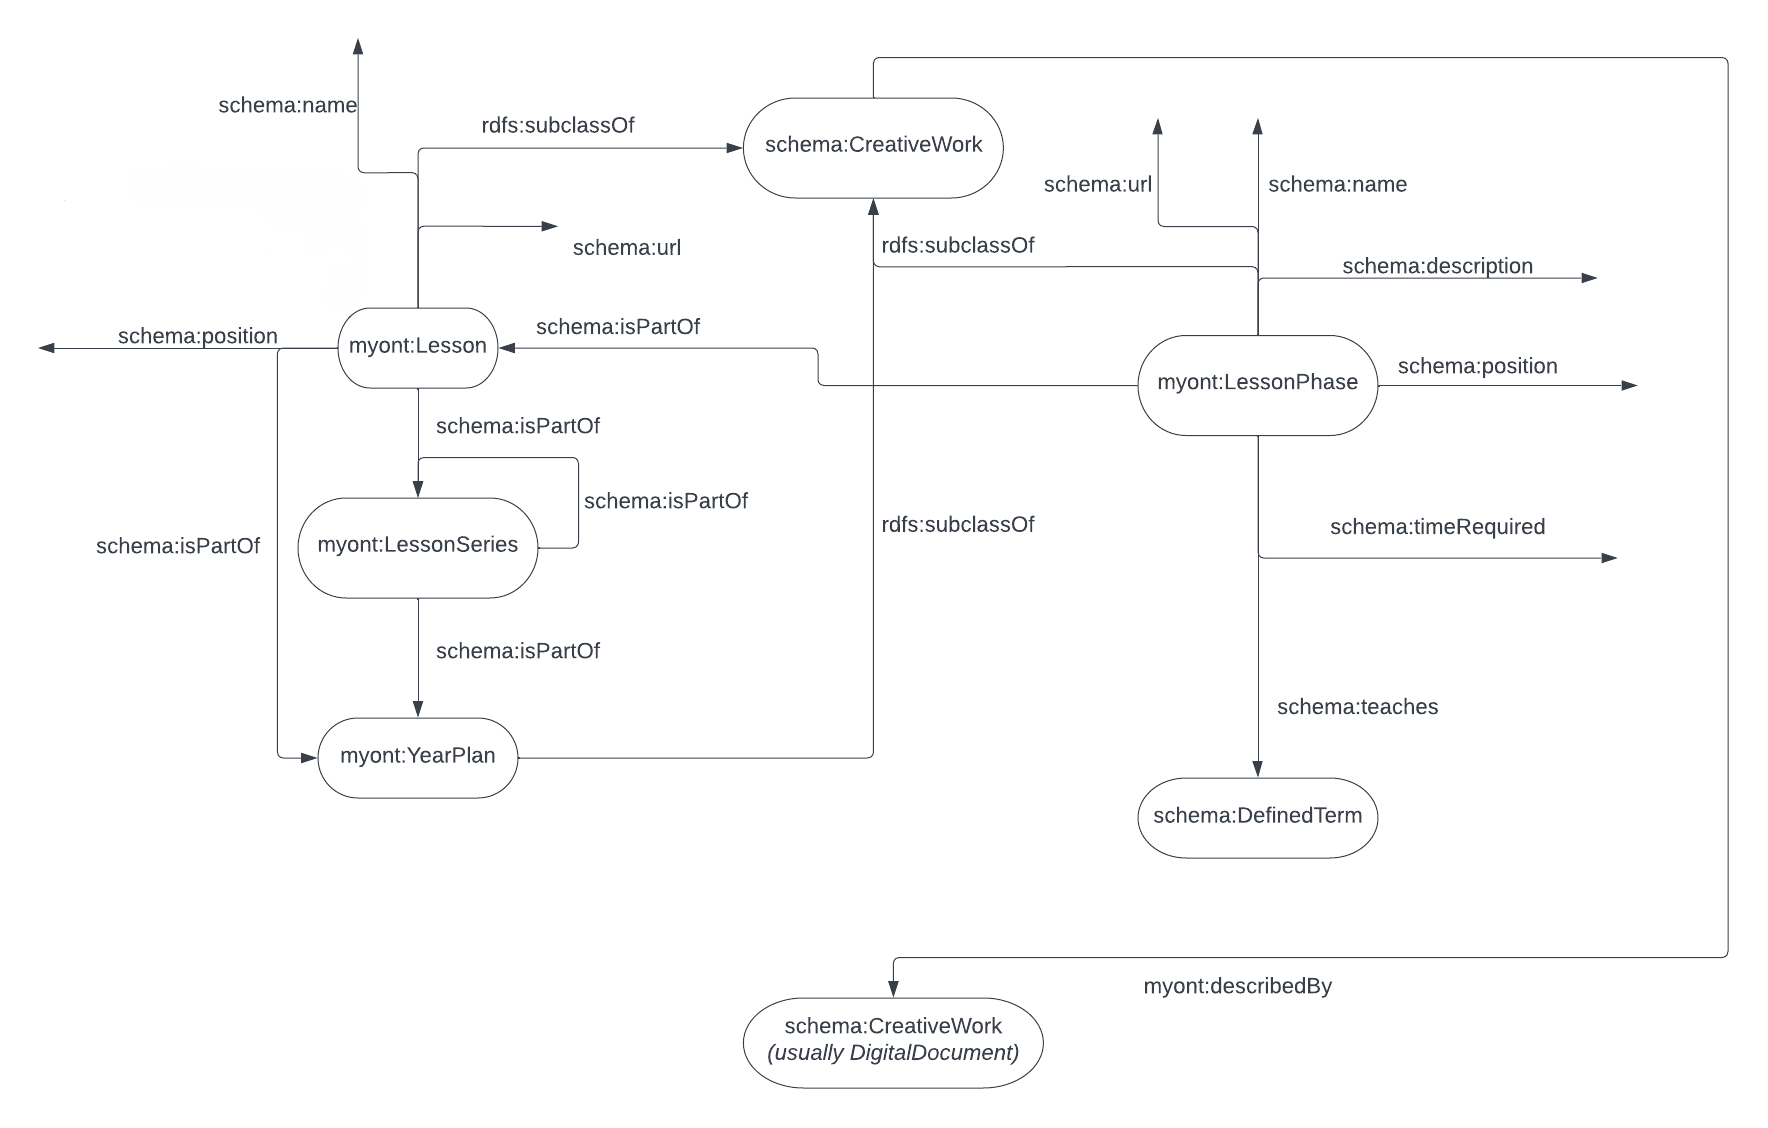
\includegraphics[scale=0.3]{uml-lessons.png}
	\end{figure}
	\noindent Nieuwe klassen werden geïntroduceerd omdat Schema.org niet genoeg semantisch onderscheid bood voor de verschillende concepten.
	Al deze klassen erven van \textit{schema:CreativeWork}.\\
	Om granulariteit en dataconsistentie te garanderen, moet een hiërarchie gerespecteerd worden: lesfasen zijn deel van lessen, lessen zijn deel van lessenreeksen en lessenreeksen zijn deel van een jaarplan.\\
	Om flexibiliteit aan te bieden bij het beschrijven van deze concepten, kan elke geïntroduceerde klasse de eigenschap \textit{myont:describedBy} hebben, wat wijst naar een document die de les, lesfase, lessenreeks of jaarplan beschrijft.

	\subsection{Cursussen}
	\noindent Zoals vermeld hebben de concepten uit subsectie \ref{subsection:yearplan} geen temporale data.
	Om aan te geven welke lessen wanneer gegeven worden, wordt het model uit figuur \ref{fig:uml-courses} gebruikt.

	\begin{figure}[h]
		\caption{Modelleren van cursussen}
		\label{fig:uml-courses}
		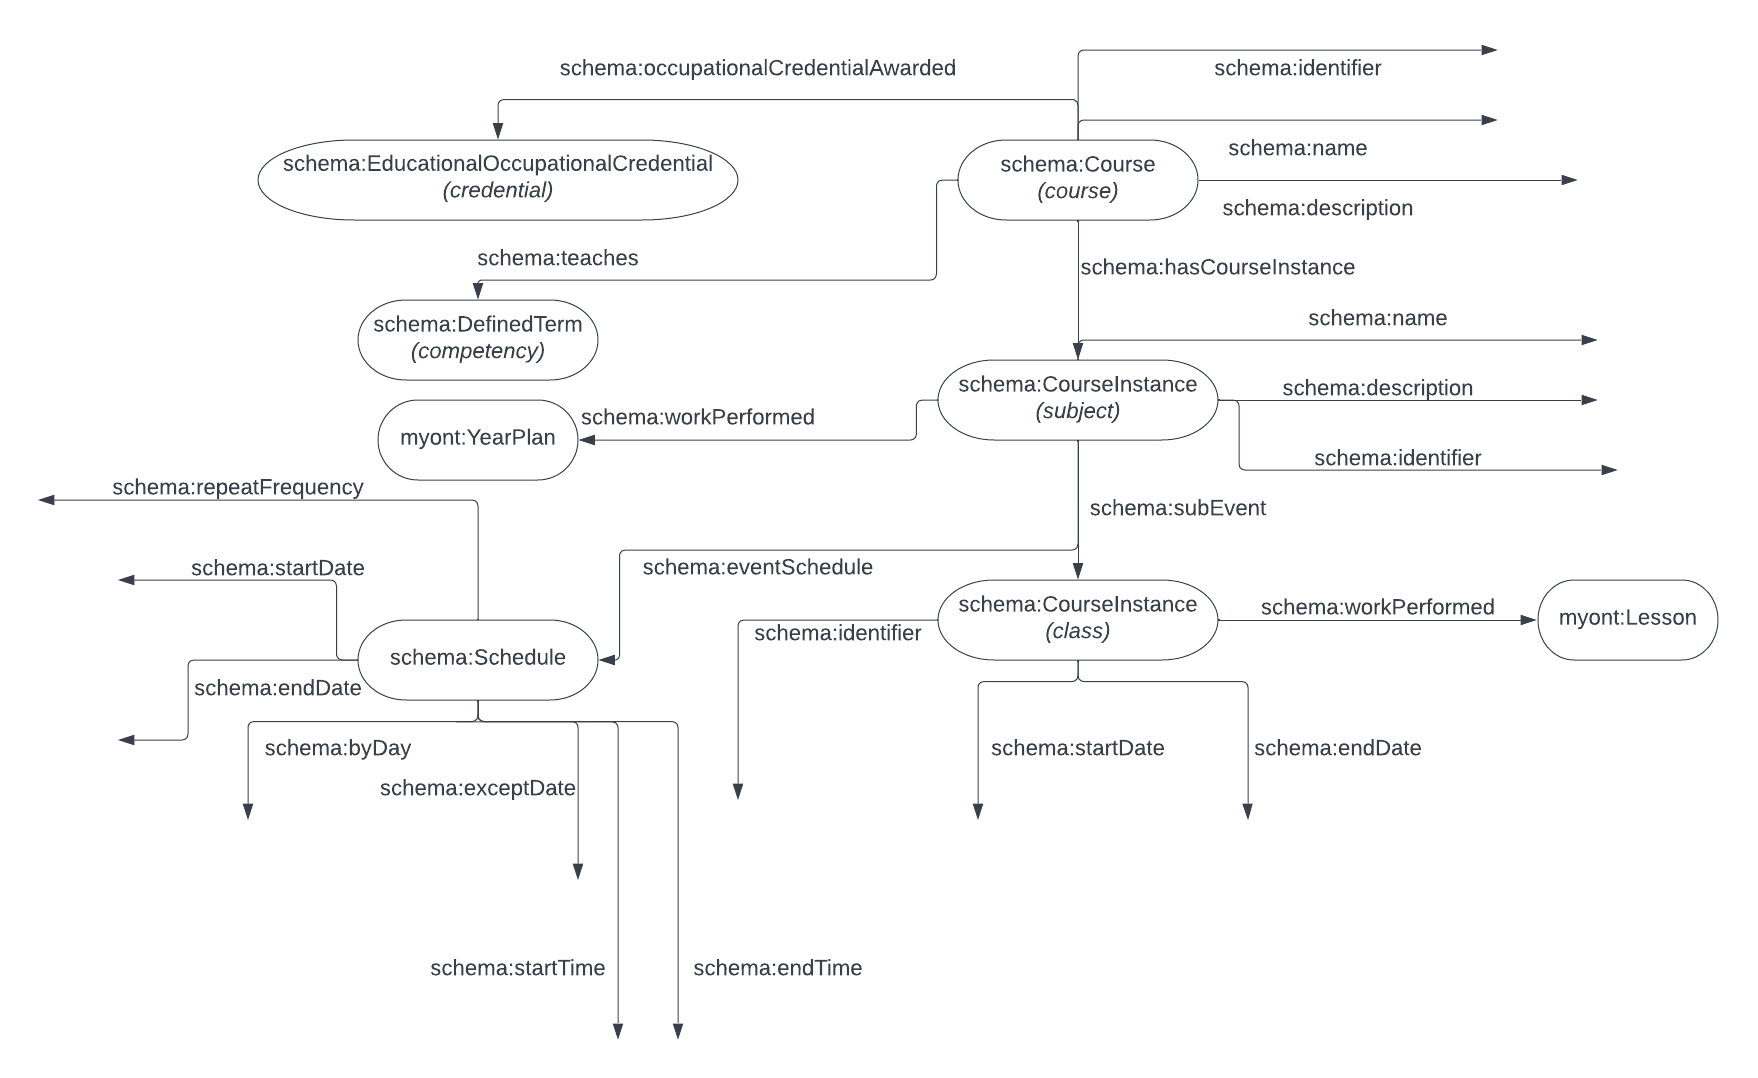
\includegraphics[scale=0.35]{uml-courses.png}
	\end{figure}
	\noindent Een cursus (`course') is een verzameling competenties dat gegeven wordt door een leerkracht aan een groep leerlingen.
	Vakken (`subject') kunnen geïnstantieerd worden die de temporale data bevatten van de cursus. Vakken hebben schema's die aangeven wanneer de leringen vallen.
	Typisch zal een nieuw vak gemaakt worden voor elk schooljaar.
	Een lering is een continue tijdsperiode waarin een leerkracht een les geeft aan een groep leerlingen.
	Het woord `lering' wordt gebruikt om het onderscheid te maken met `lessen' uit subsectie \ref{subsection:yearplan}, wat geen temporale data heeft.\\
	Maximaal 1 jaarplan wordt gegeven binnen een vak, en maximaal 1 les wordt gegeven in een lering.

	\subsection{Cursusmaterialen en oefeningen}
	\noindent Het modelleren van cursusmateriaal en oefeningen wordt gedaan volgens het datamodel weergegeven in figuur \ref{fig:uml-materialdata}.

	\begin{figure}[h]
		\centering
		\caption{Modelleren van leermaterialen en oefeningen}
		\label{fig:uml-materialdata}
		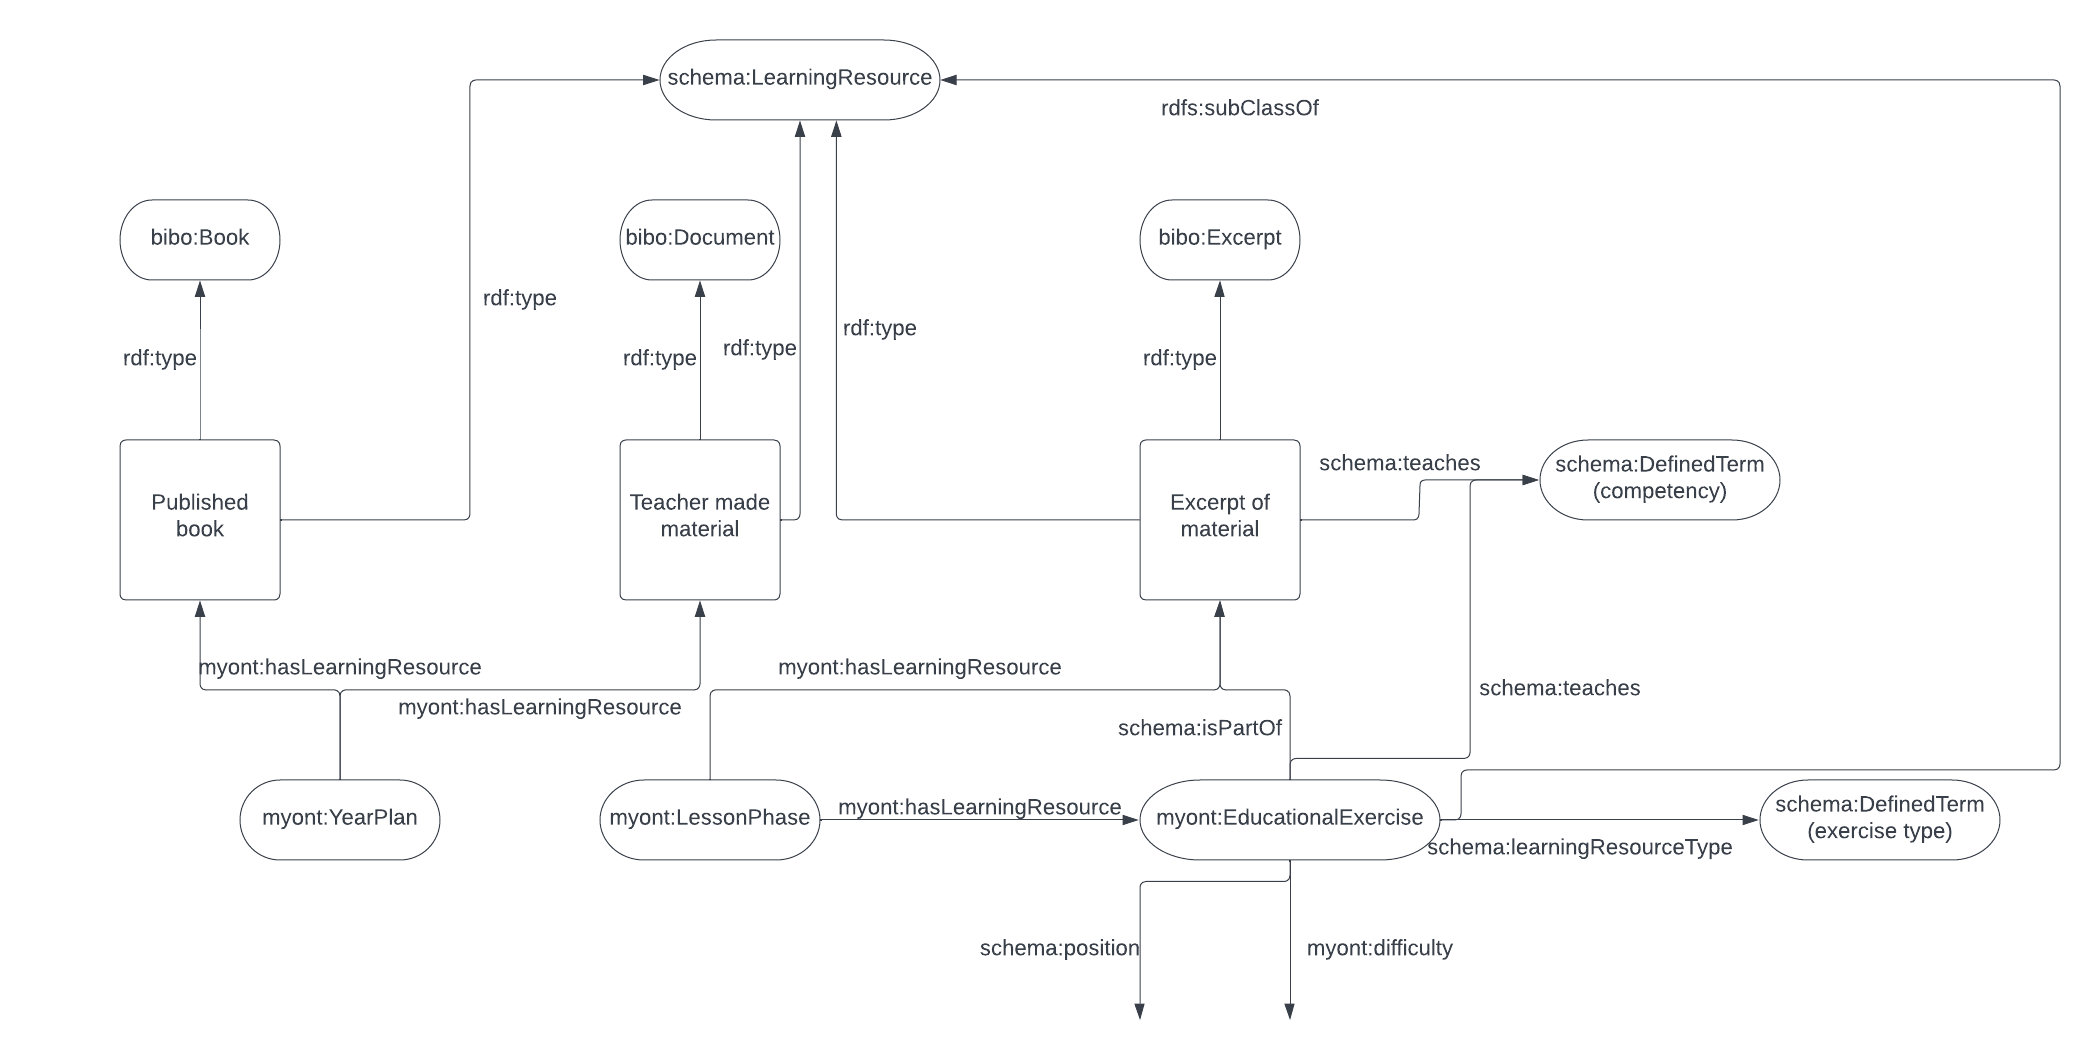
\includegraphics[scale=0.25]{uml-materialdata.png}
	\end{figure}
	\noindent Alle instanties die cursusmateriaal voorstellen, moeten zowel het type \textit{schema:LearningResource} en een type uit de bibo ontologie hebben.
	Dit is nodig omdat eigenschappen van Schema.org en DC gebruikt worden om deze concepten te modelleren.\\
	Een nieuwe klasse voor educatieve oefeningen werd geïntroduceerd omdat Schema.org en DC niet genoeg eigenschappen en klassen aanboden om deze te beschrijven.

	\subsection{Didactische methoden en educatieve taxonomieën}

	\noindent Een didactische methode is de manier waarop leerstof gegeven wordt.
	Er werd gekozen om deze niet apart te modelleren, maar om de belangrijke kenmerken, zoals naar voor gekomen in de interviews, ervan toe te voegen als eigenschappen van bestaande klassen.\\
	Het volledig modelleren van didactische methoden valt buiten het bestek van dit onderzoek. Een goede referentie hiervoor is Mencke, S. et al \cite{hierarchy}.\\
	Educatieve taxonomieën geven aan op welk niveau iemand leerstof beheerst.
	Dit werd gemodelleerd met Schema.org, zoals aangegeven in figuur \ref{fig:uml-dm}.

	\begin{figure}[h]
		\caption{Modelleren van didactische methoden en educatieve taxonomieën}
		\label{fig:uml-dm}
		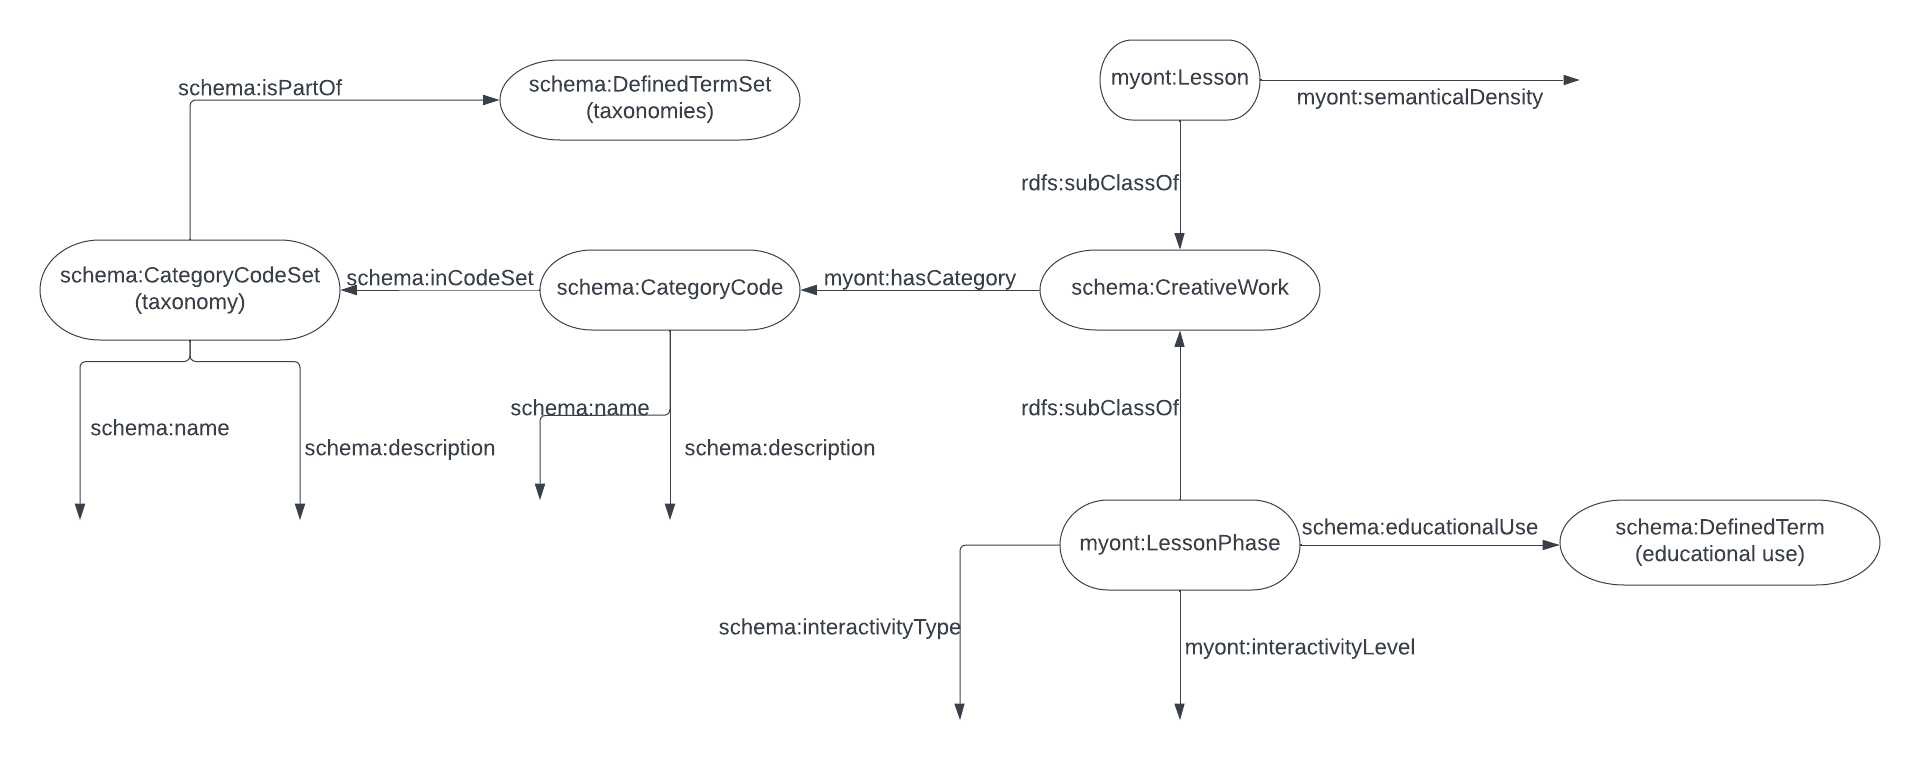
\includegraphics[scale=0.3]{uml-taxonomies.png}
	\end{figure}

\section{Conclusie}

\noindent De meeste problemen uit subsectie \ref{subsection:existing-tools} worden opgelost door de gedecentralizeerde aard van gelinkte data.
Deze data kan door verschillende instanties onderhouden worden, wat betekent dat als de servers van een bedrijf falen, enkel de leerkrachten die hun data daar opslaan geraakt worden. 
Wanneer een leerkracht verandert van bedrijf, zal de data niet verloren gaan.\\
Leerkrachten hoeven ook niet alle gegevens zelf in te vullen. Uitgevers kunnen bijvoorbeeld data over hun studieboeken publiceren.\\ \\
Door competenties te modelleren als \textit{schema:DefinedTerm} kan men gebruikmaken van de officiële data van de overheid zonder rekening te moeten houden met de onderliggende ontologie.
Dit betekent dat dit model bruikbaar is voor elk educatief systeem dat gebaseerd is op competenties.\\ \\
Door de klasse \textit{myont:LessonPhase} te introduceren, is er meer granulariteit. Deze fasen kunnen indien nodig tussen de lessen worden verplaatst.\\
De competentievragen die uit de interviews zijn gehaald, vertegenwoordigen overzichten die de geïnterviewden nuttig achtten.
Door het opstellen van bijhorende SPARQL-query's wordt aangetoond dat deze overzichten aan leerkrachten kunnen worden aangeboden.

\section*{Dankwoord}
\noindent Ik dank Thomas Delva en Dr.ir. Ben De Meester (Universiteit Gent) voor hun intensieve begeleiding bij de ontwikkeling van dit model.
Ook een dank aan Prof. dr. Kris Coolsaet (Universiteit Gent) voor het helpen met het educatieve luik van het onderzoek.
Ook bedankt aan alle leerkrachten die tijd vrijmaakten om een interview af te nemen.\\
Een speciale dank aan Prof. dr. ir. Ruben Verborgh (Universiteit Gent) voor het aanwakkeren van mijn interesse in linked data.
Ook een speciale dank aan de Universiteit van Gent voor de kwalitatieve opleiding en mij in staat te stellen dit interessante onderzoek te voeren.


\bibliographystyle{IEEEtran}
\bibliography{../bibliography}
\end{document}